\section{Evaluation}
\label{sec:evaluation}

% TODO: Setting.  Computer resources (CPU, RAM, OS).

\subsection{Setup}

We have evaluated our implementation in an environment consisting on two
computers located in the same gigabit ethernet network.  We run the Broker,
Third Party and one Subscriber on the first computer, and all the Publishers in
the second computer.  We perform all the analysis on the performance of several
operations in the Broker and Third Party, which run together in a computer
running Linux with an Intel Core i7-6600U CPU with 16GB of RAM.  In order to
avoid isolate the performance influence of the Broker and the Third Party, we
have serialized the garbling and evaluation of the garbled circuit operations,
mimicking the situation in which the Broker and Third Party are run on
different servers.

\subsection{Microbenchmarks}

We have selected 5 numerical operations of varying complexity (\emph{summation,
multiplicatory, mean, variance, minimum}) to evaluate the cost of the different
parts of our implementation.  We securely evaluate these functions over the values (encoded as 32 bit fixed point numbers) received from a variable number of Publishers.

% Plots

\begin{figure}
  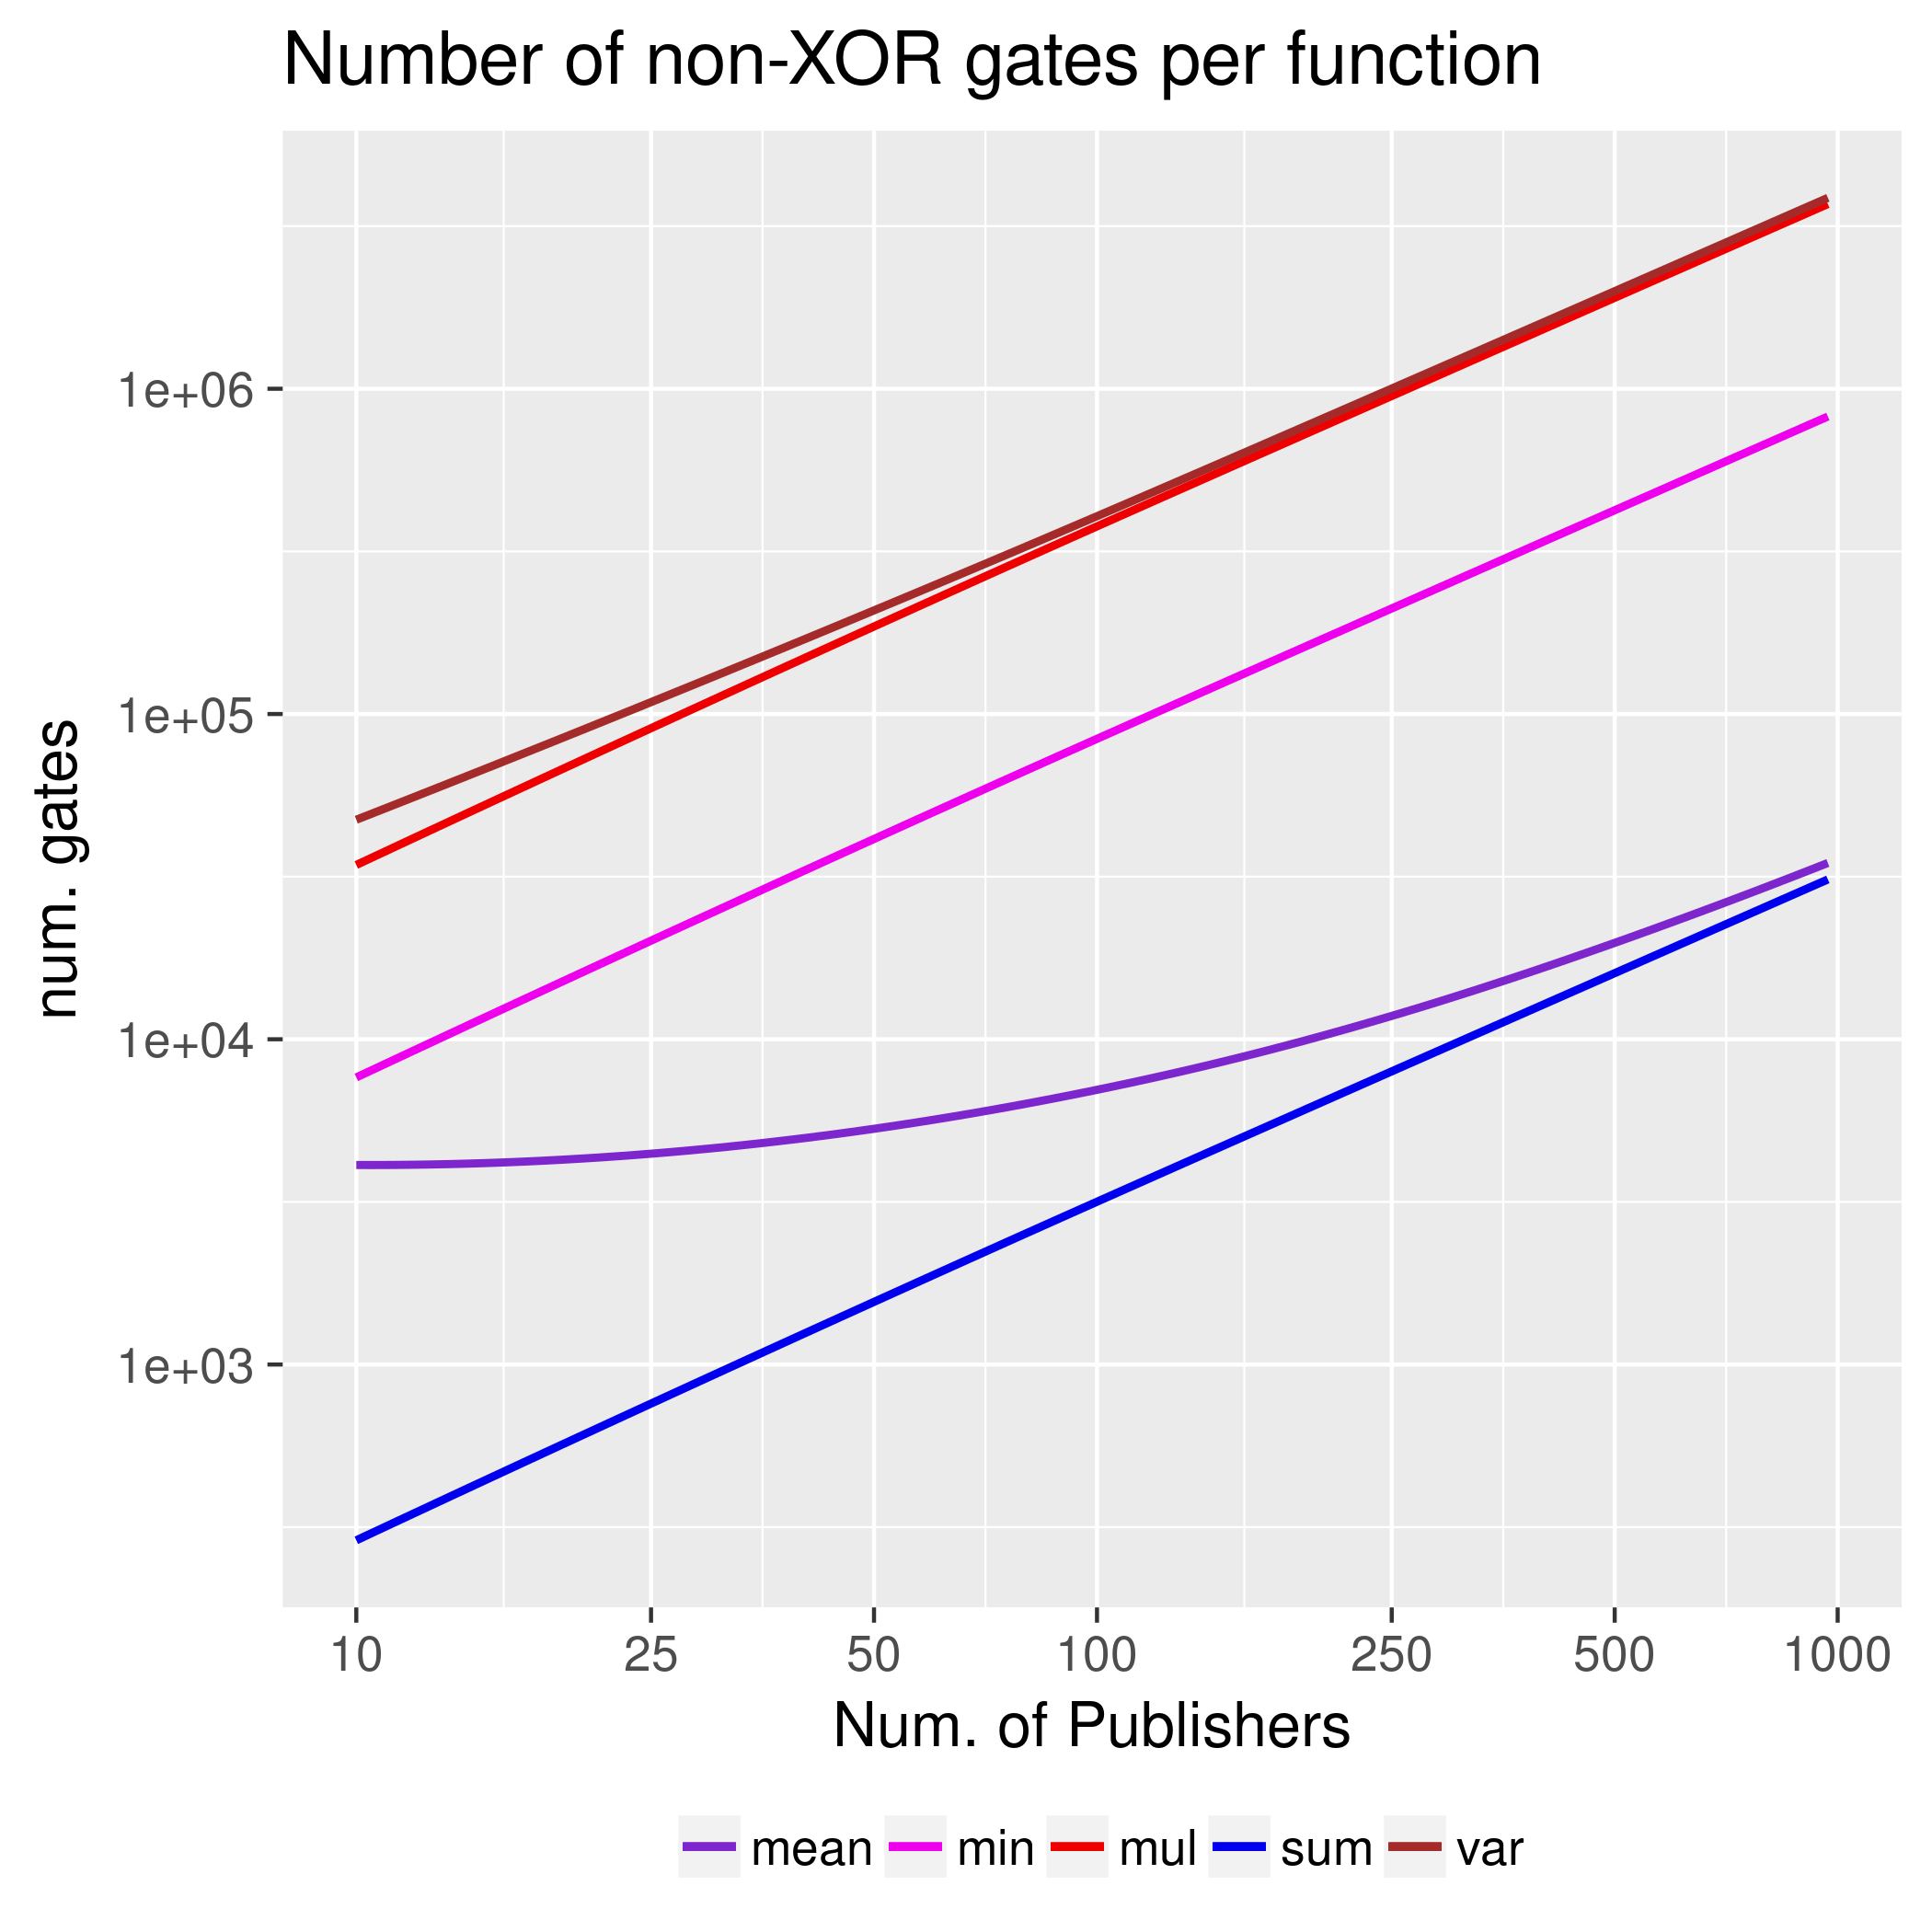
\includegraphics[width=0.5\textwidth]{plots/gates_log.png}
  \caption{Gates count per function used in the microbenchmarks.}
\end{figure}

\begin{figure}
  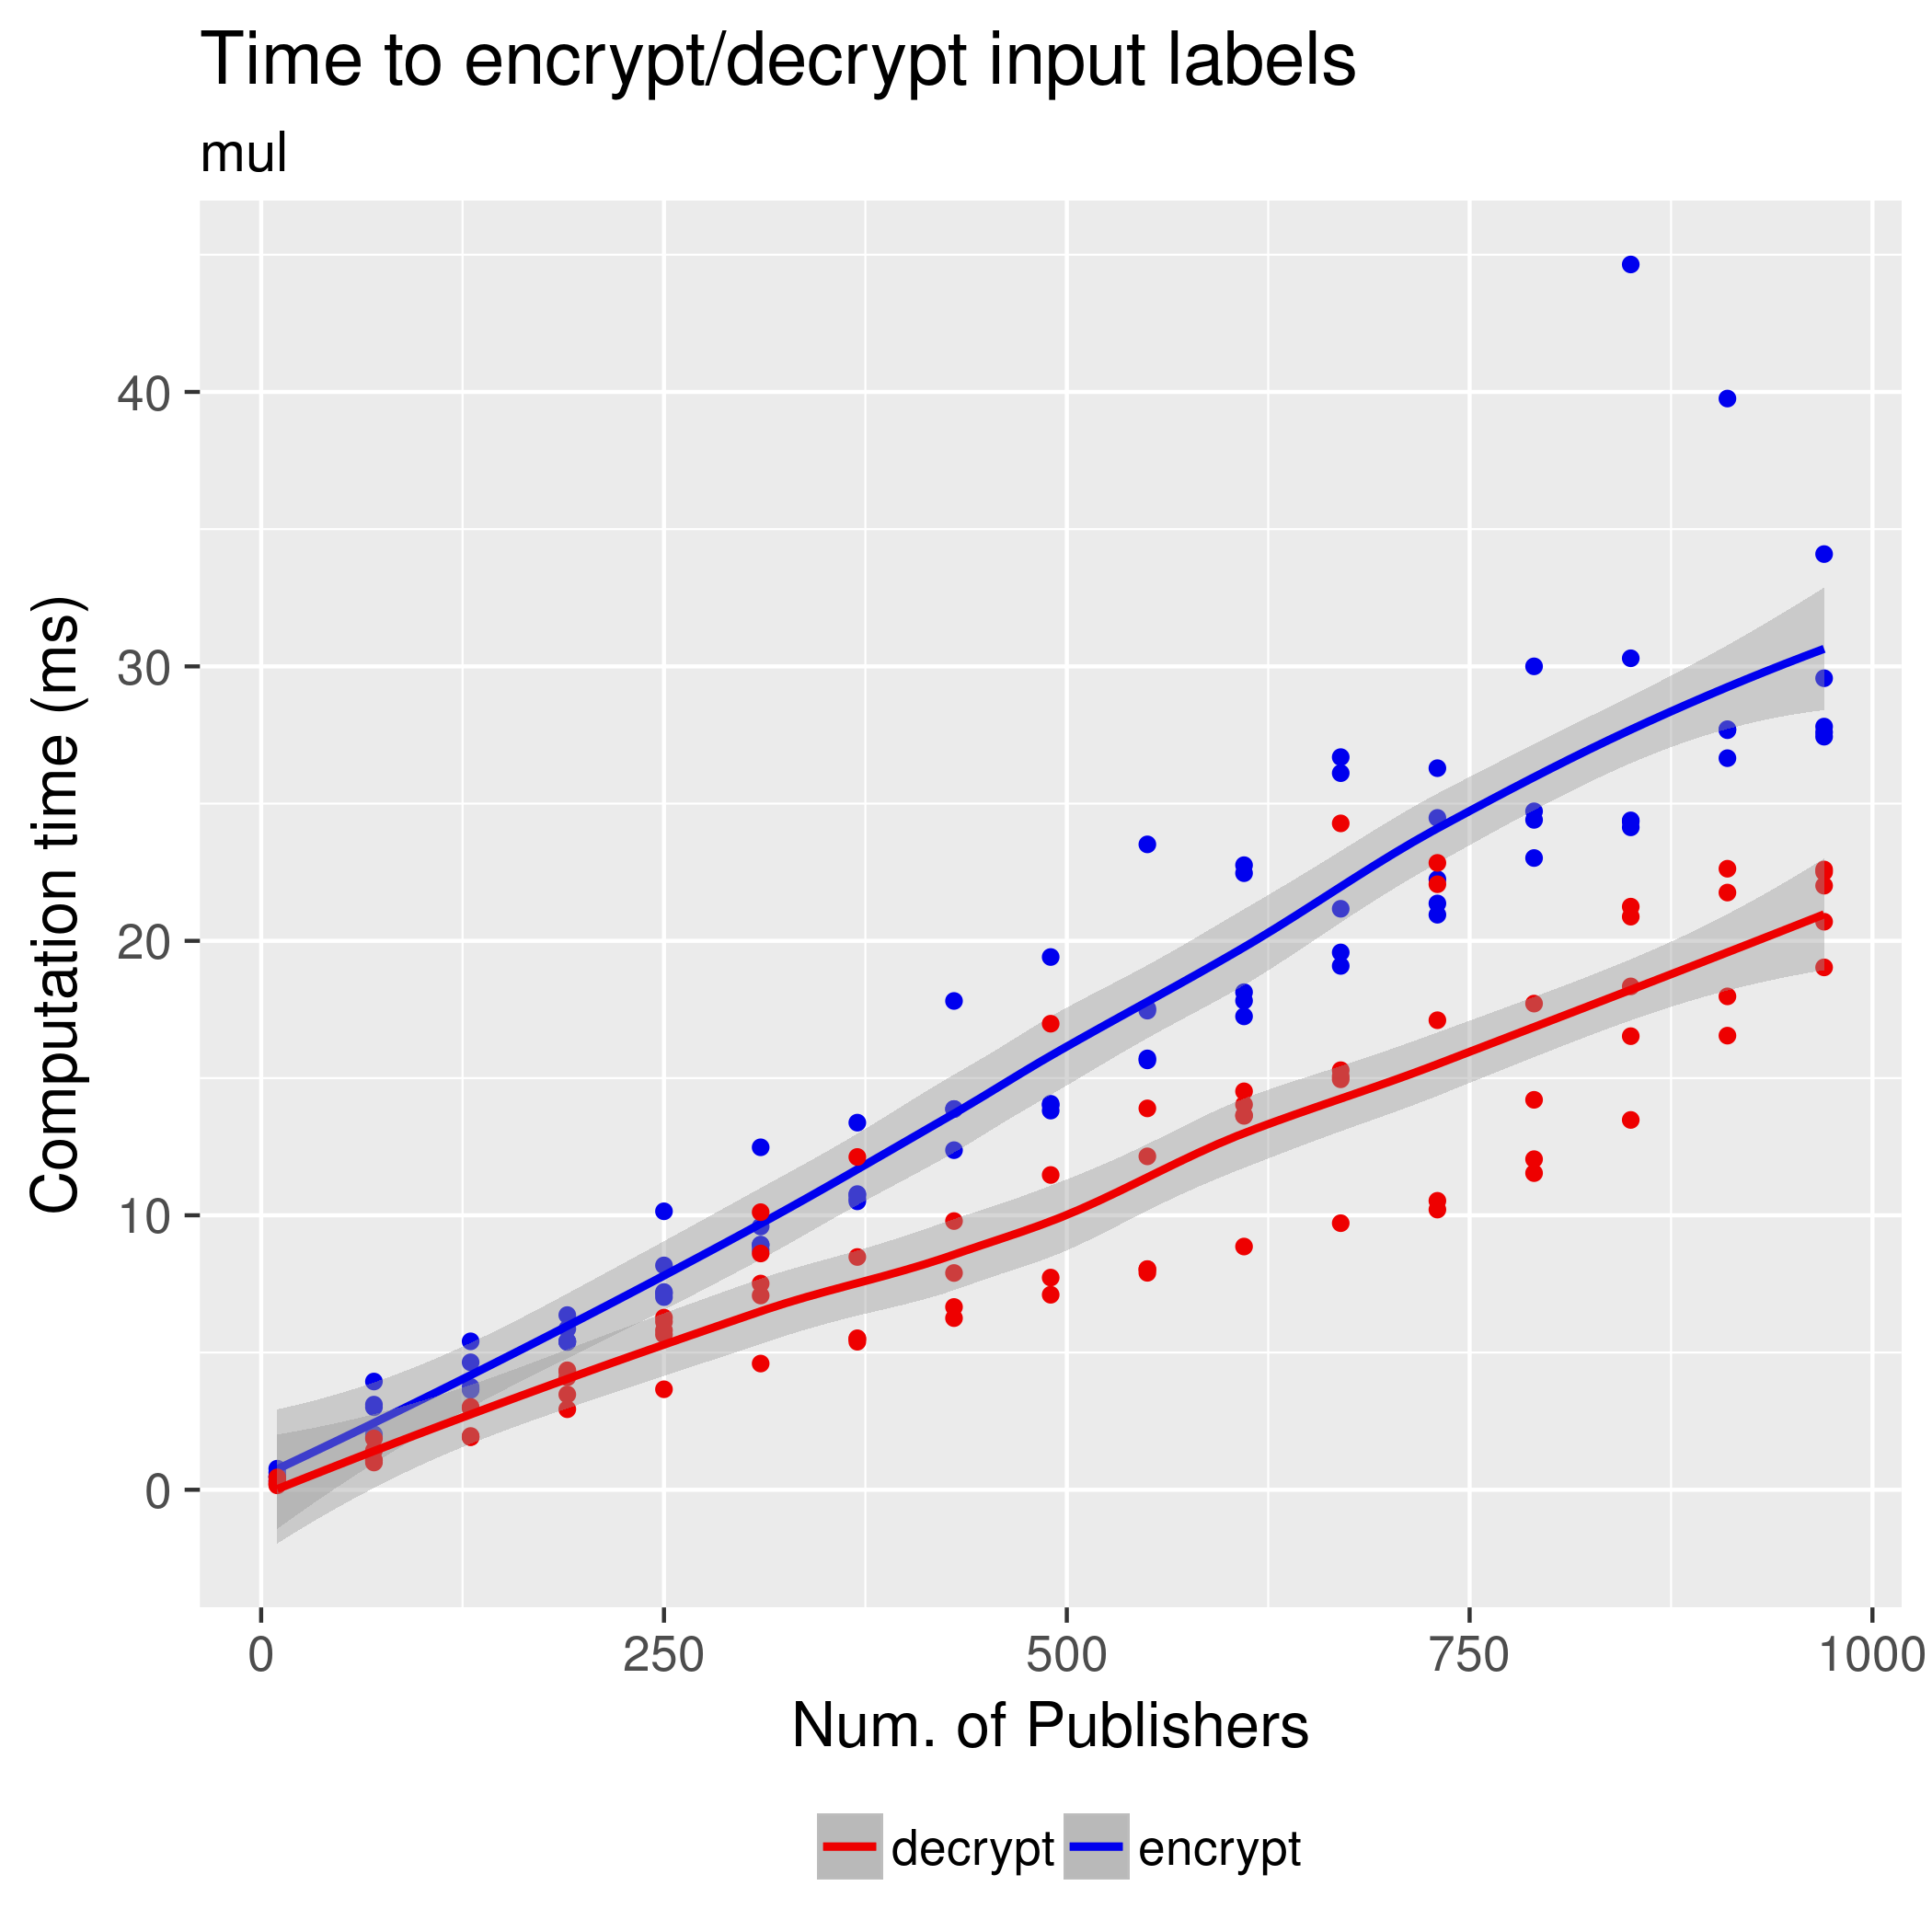
\includegraphics[width=0.5\textwidth]{plots/enc_dec_inputs.png}
  \caption{Time spent garbling and evaluating the identity input gates.}
\end{figure}

\begin{figure}
  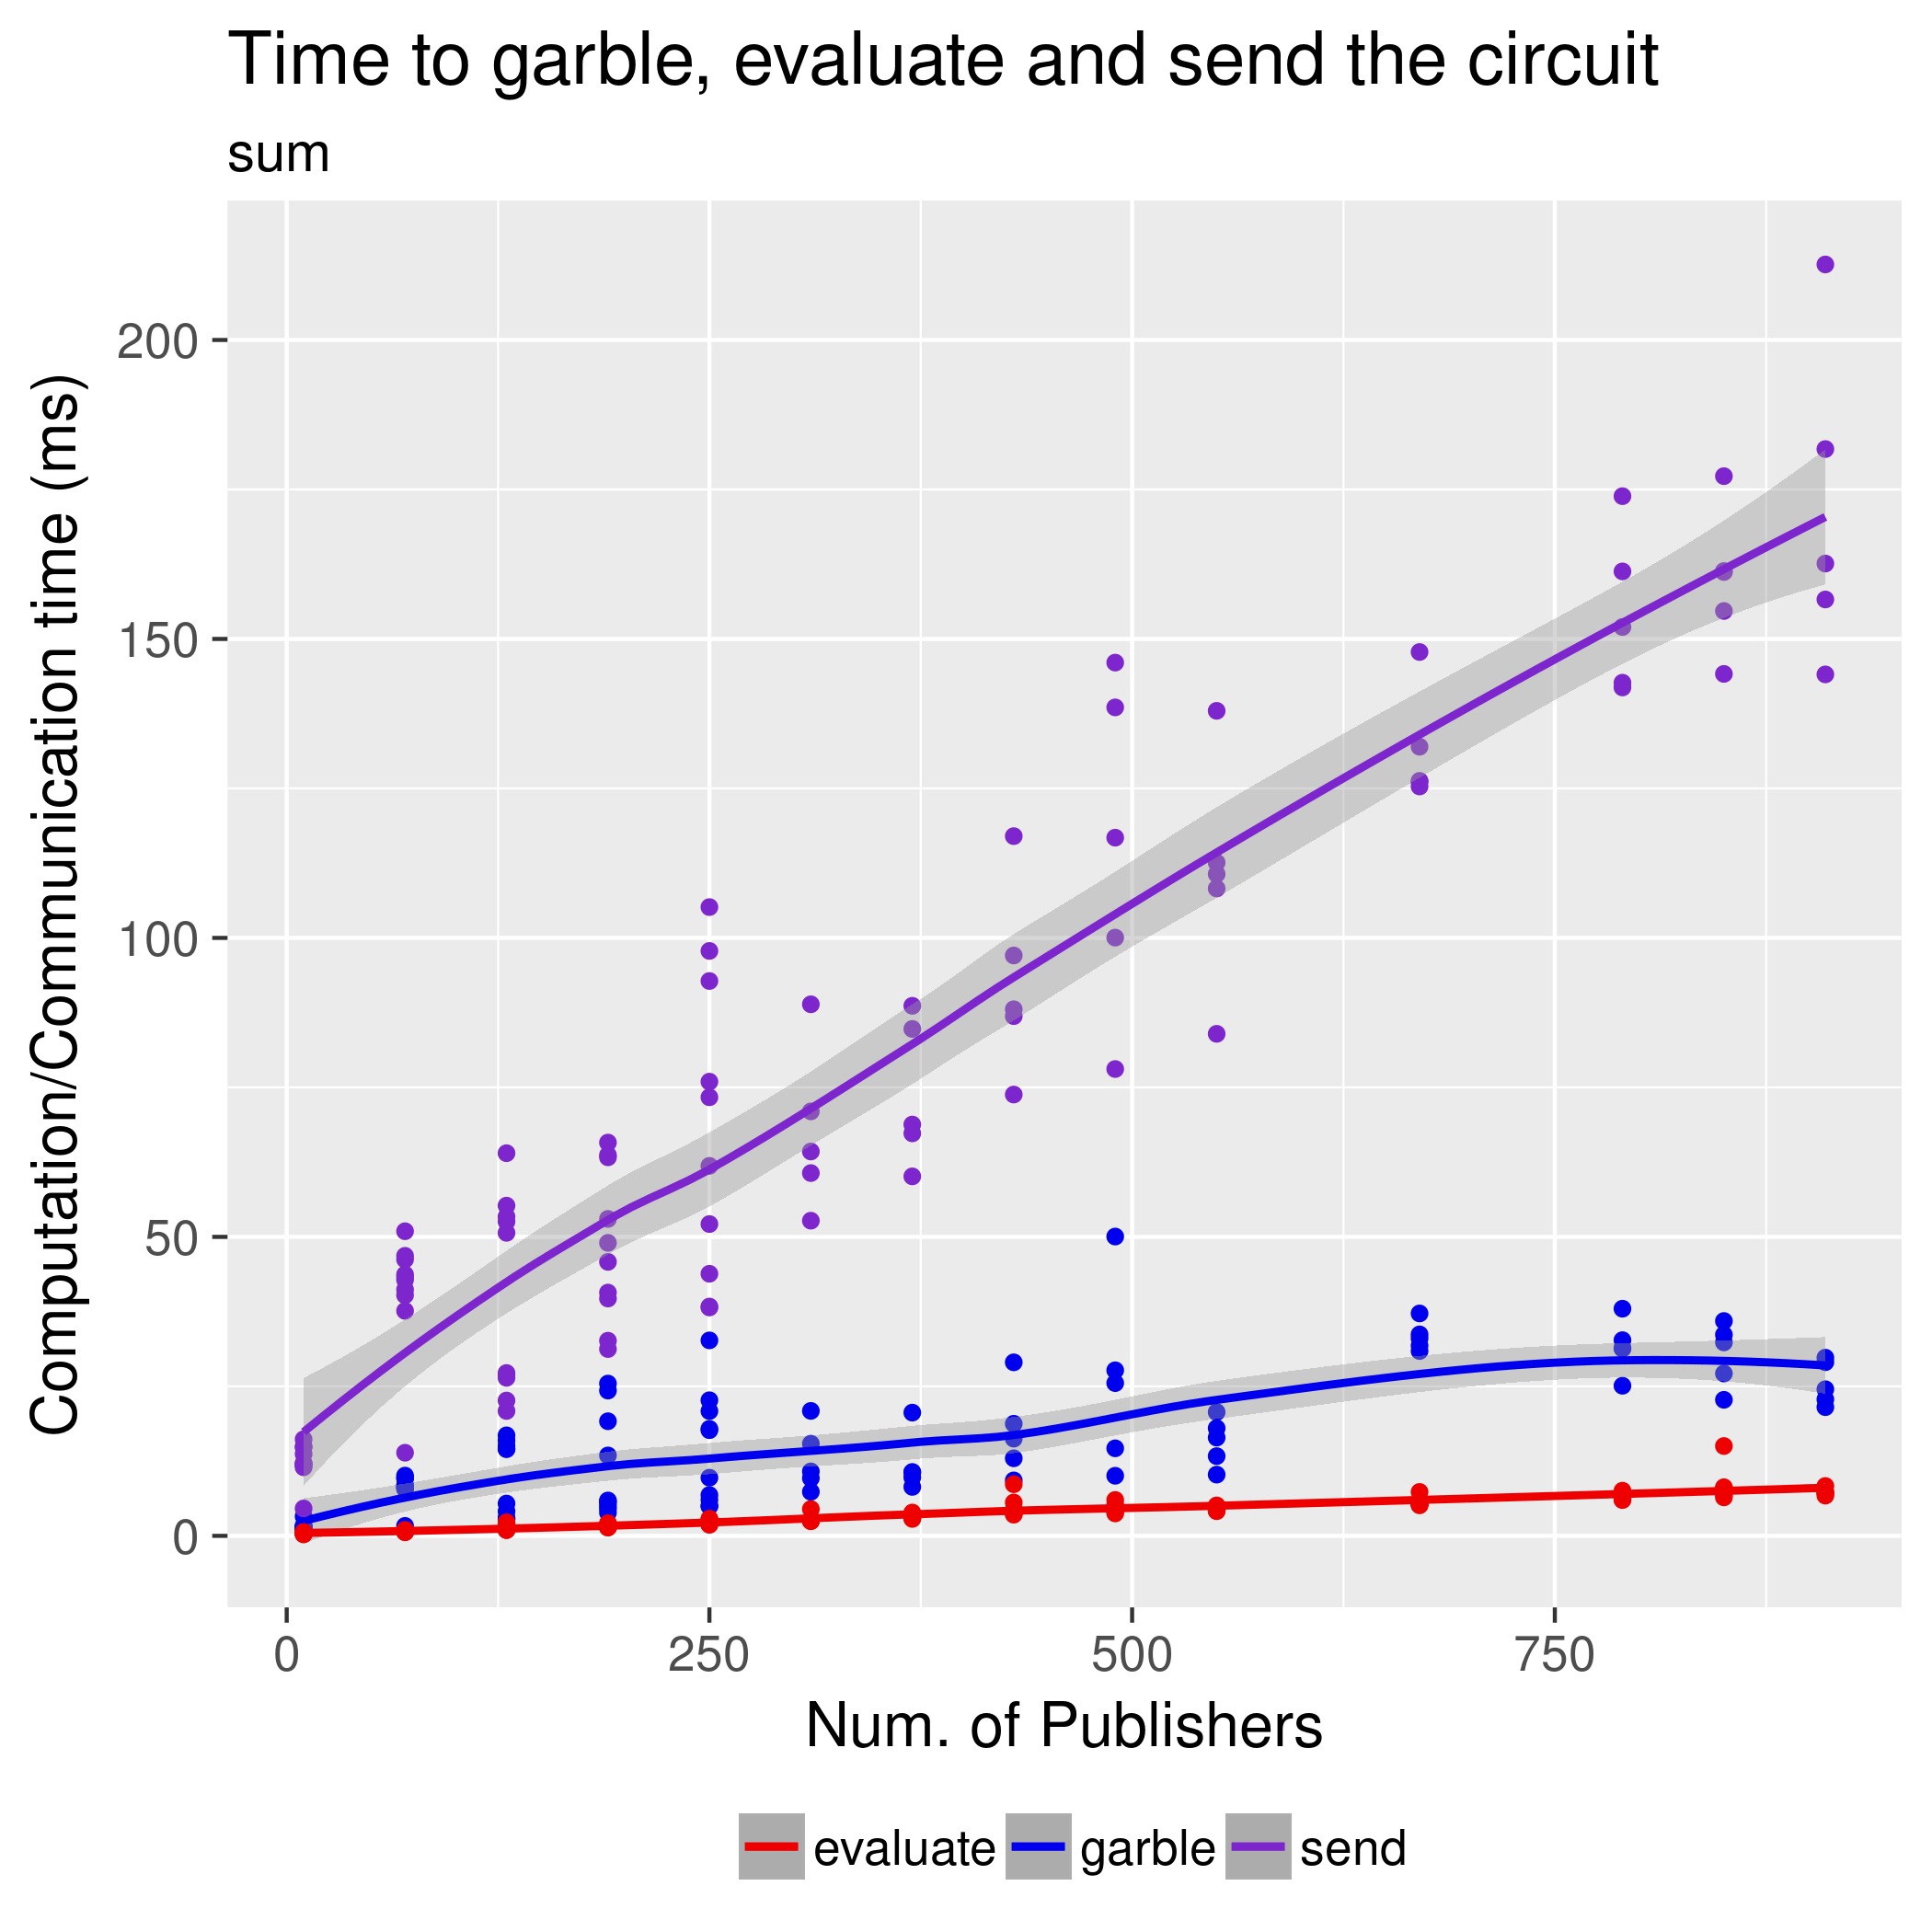
\includegraphics[width=0.5\textwidth]{plots/sum_circuit_2017-05-15.png}
  \caption{Time spent garbling the circuit, sending the result to the Broker and evaluating it.}
\end{figure}

%\begin{figure}
%  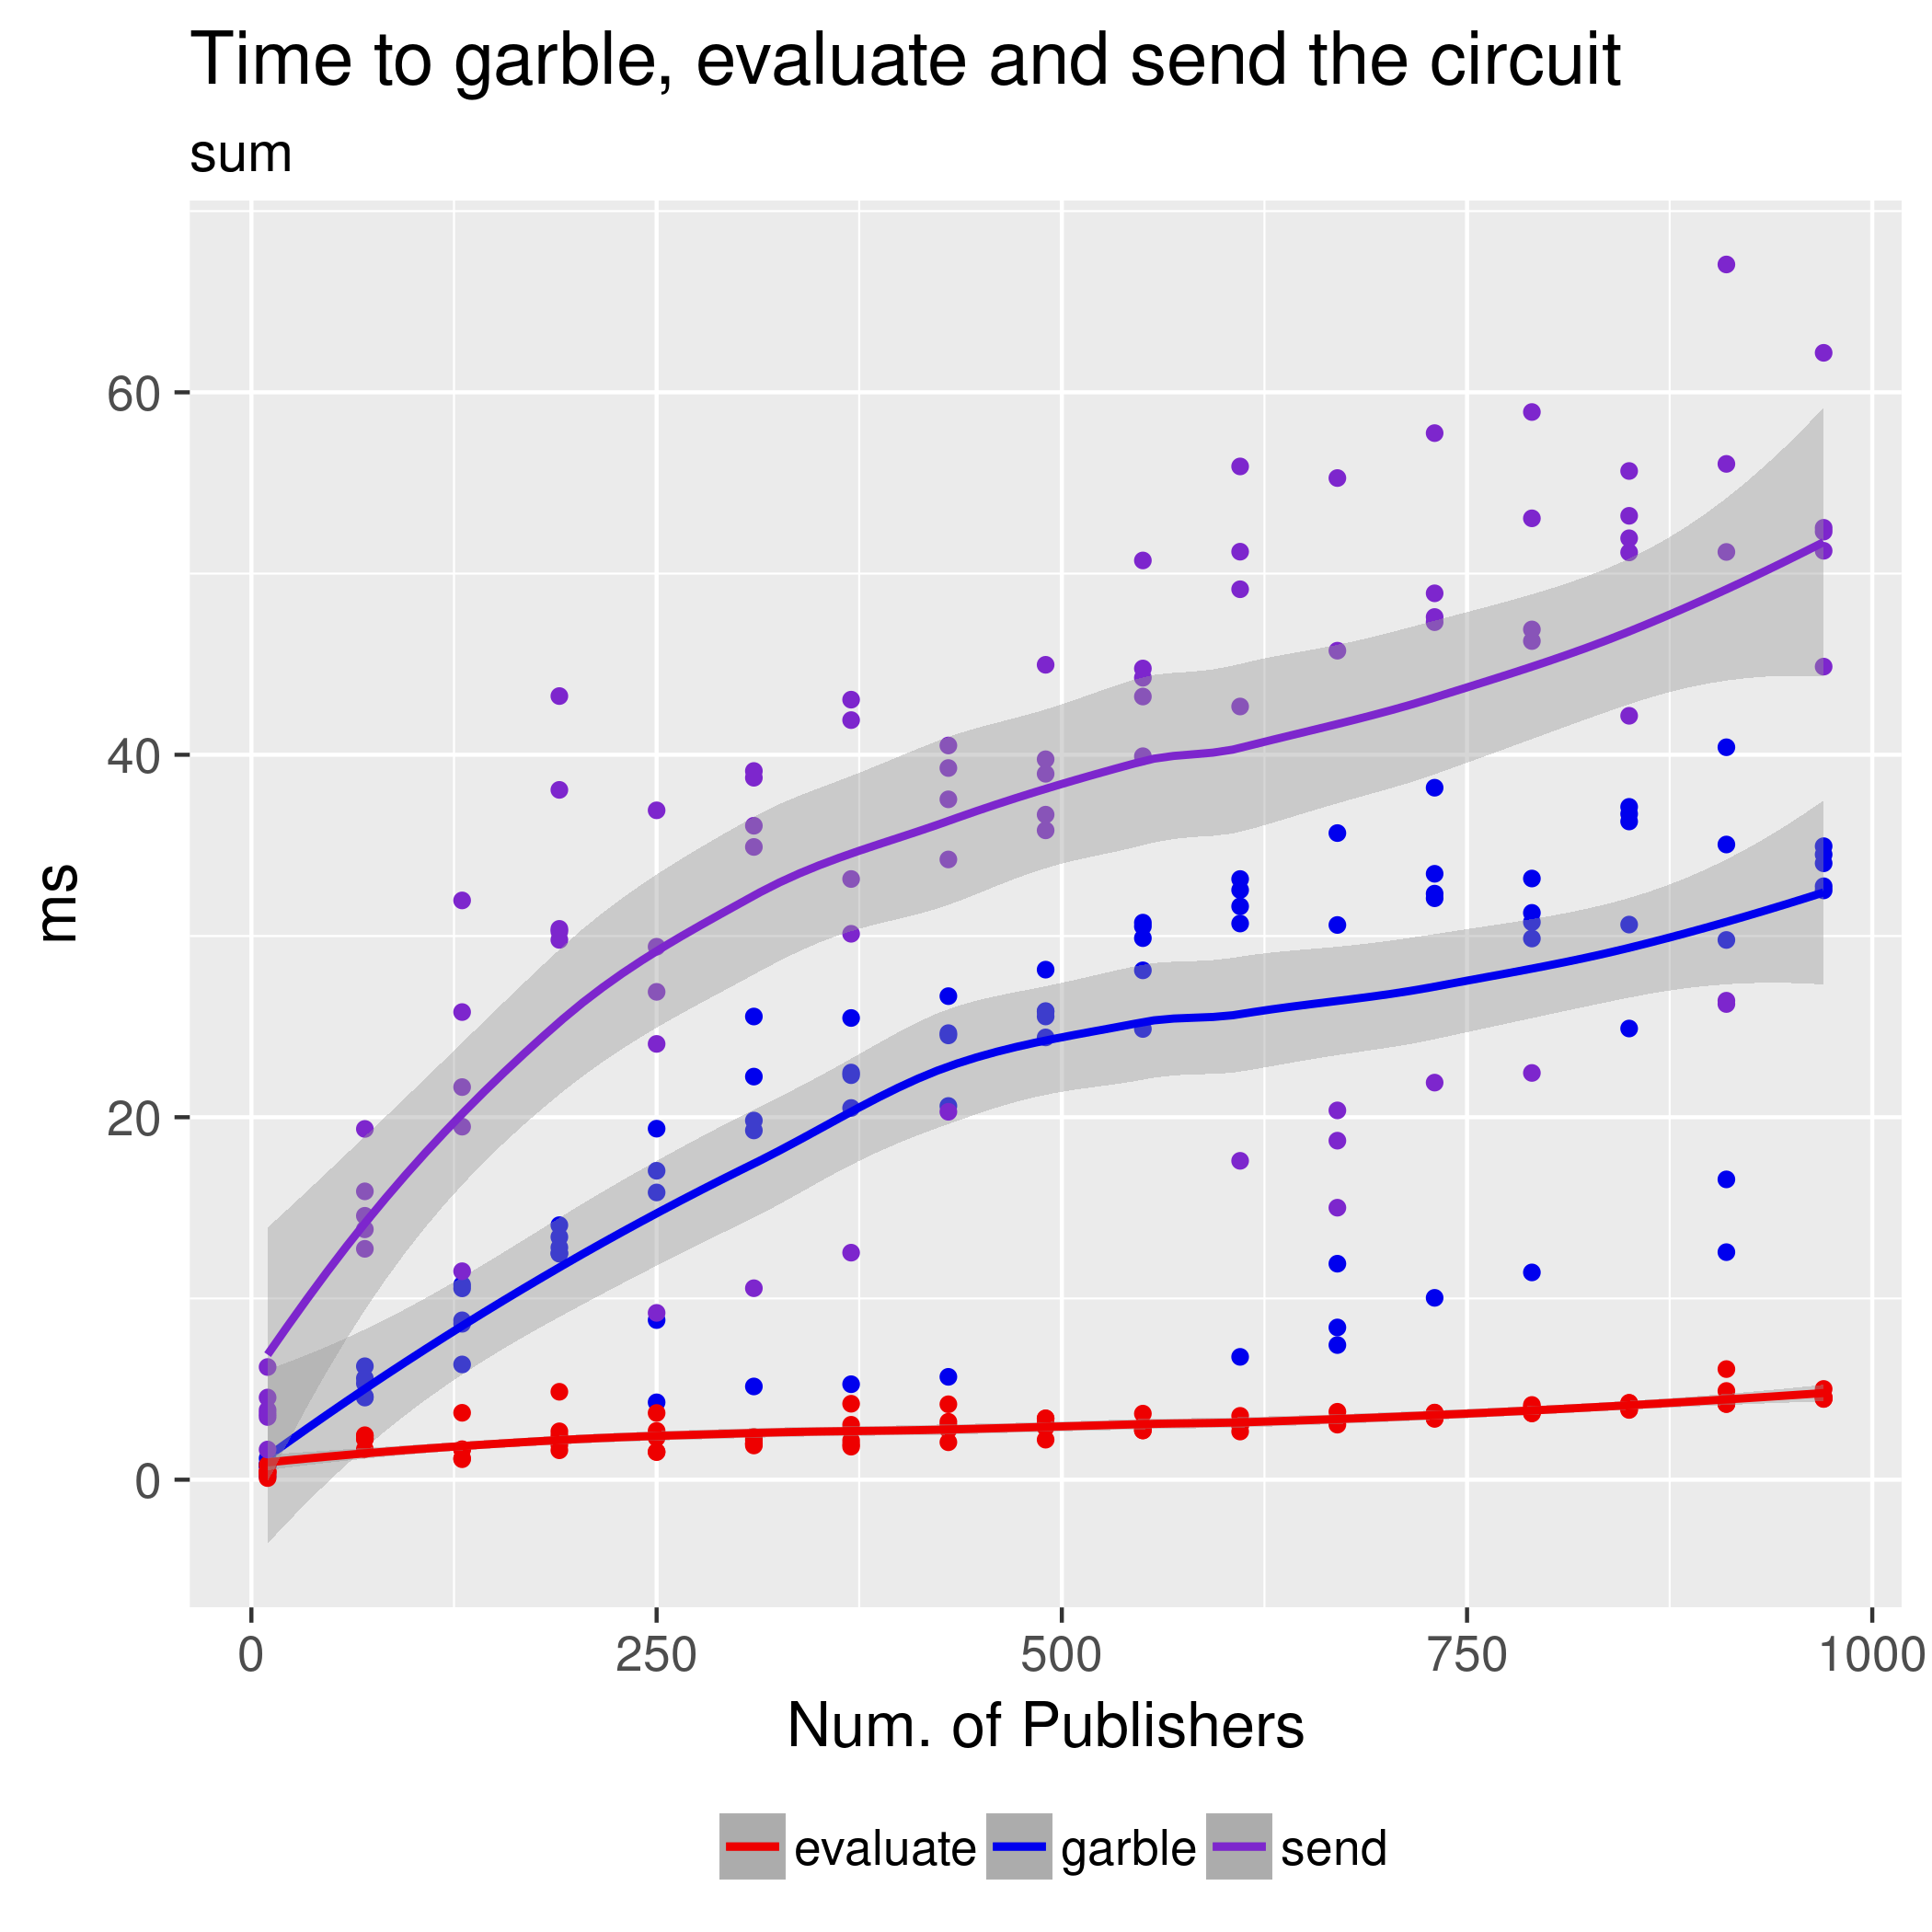
\includegraphics[width=0.5\textwidth]{plots/sum_circuit_onepub_2017-05-13.png}
%  \caption{Time spent garbling the circuit, sending the result to the Broker
%  and evaluating it removing the overhead of handling the Publishers
%  connections.}
%\end{figure}

\begin{figure}
  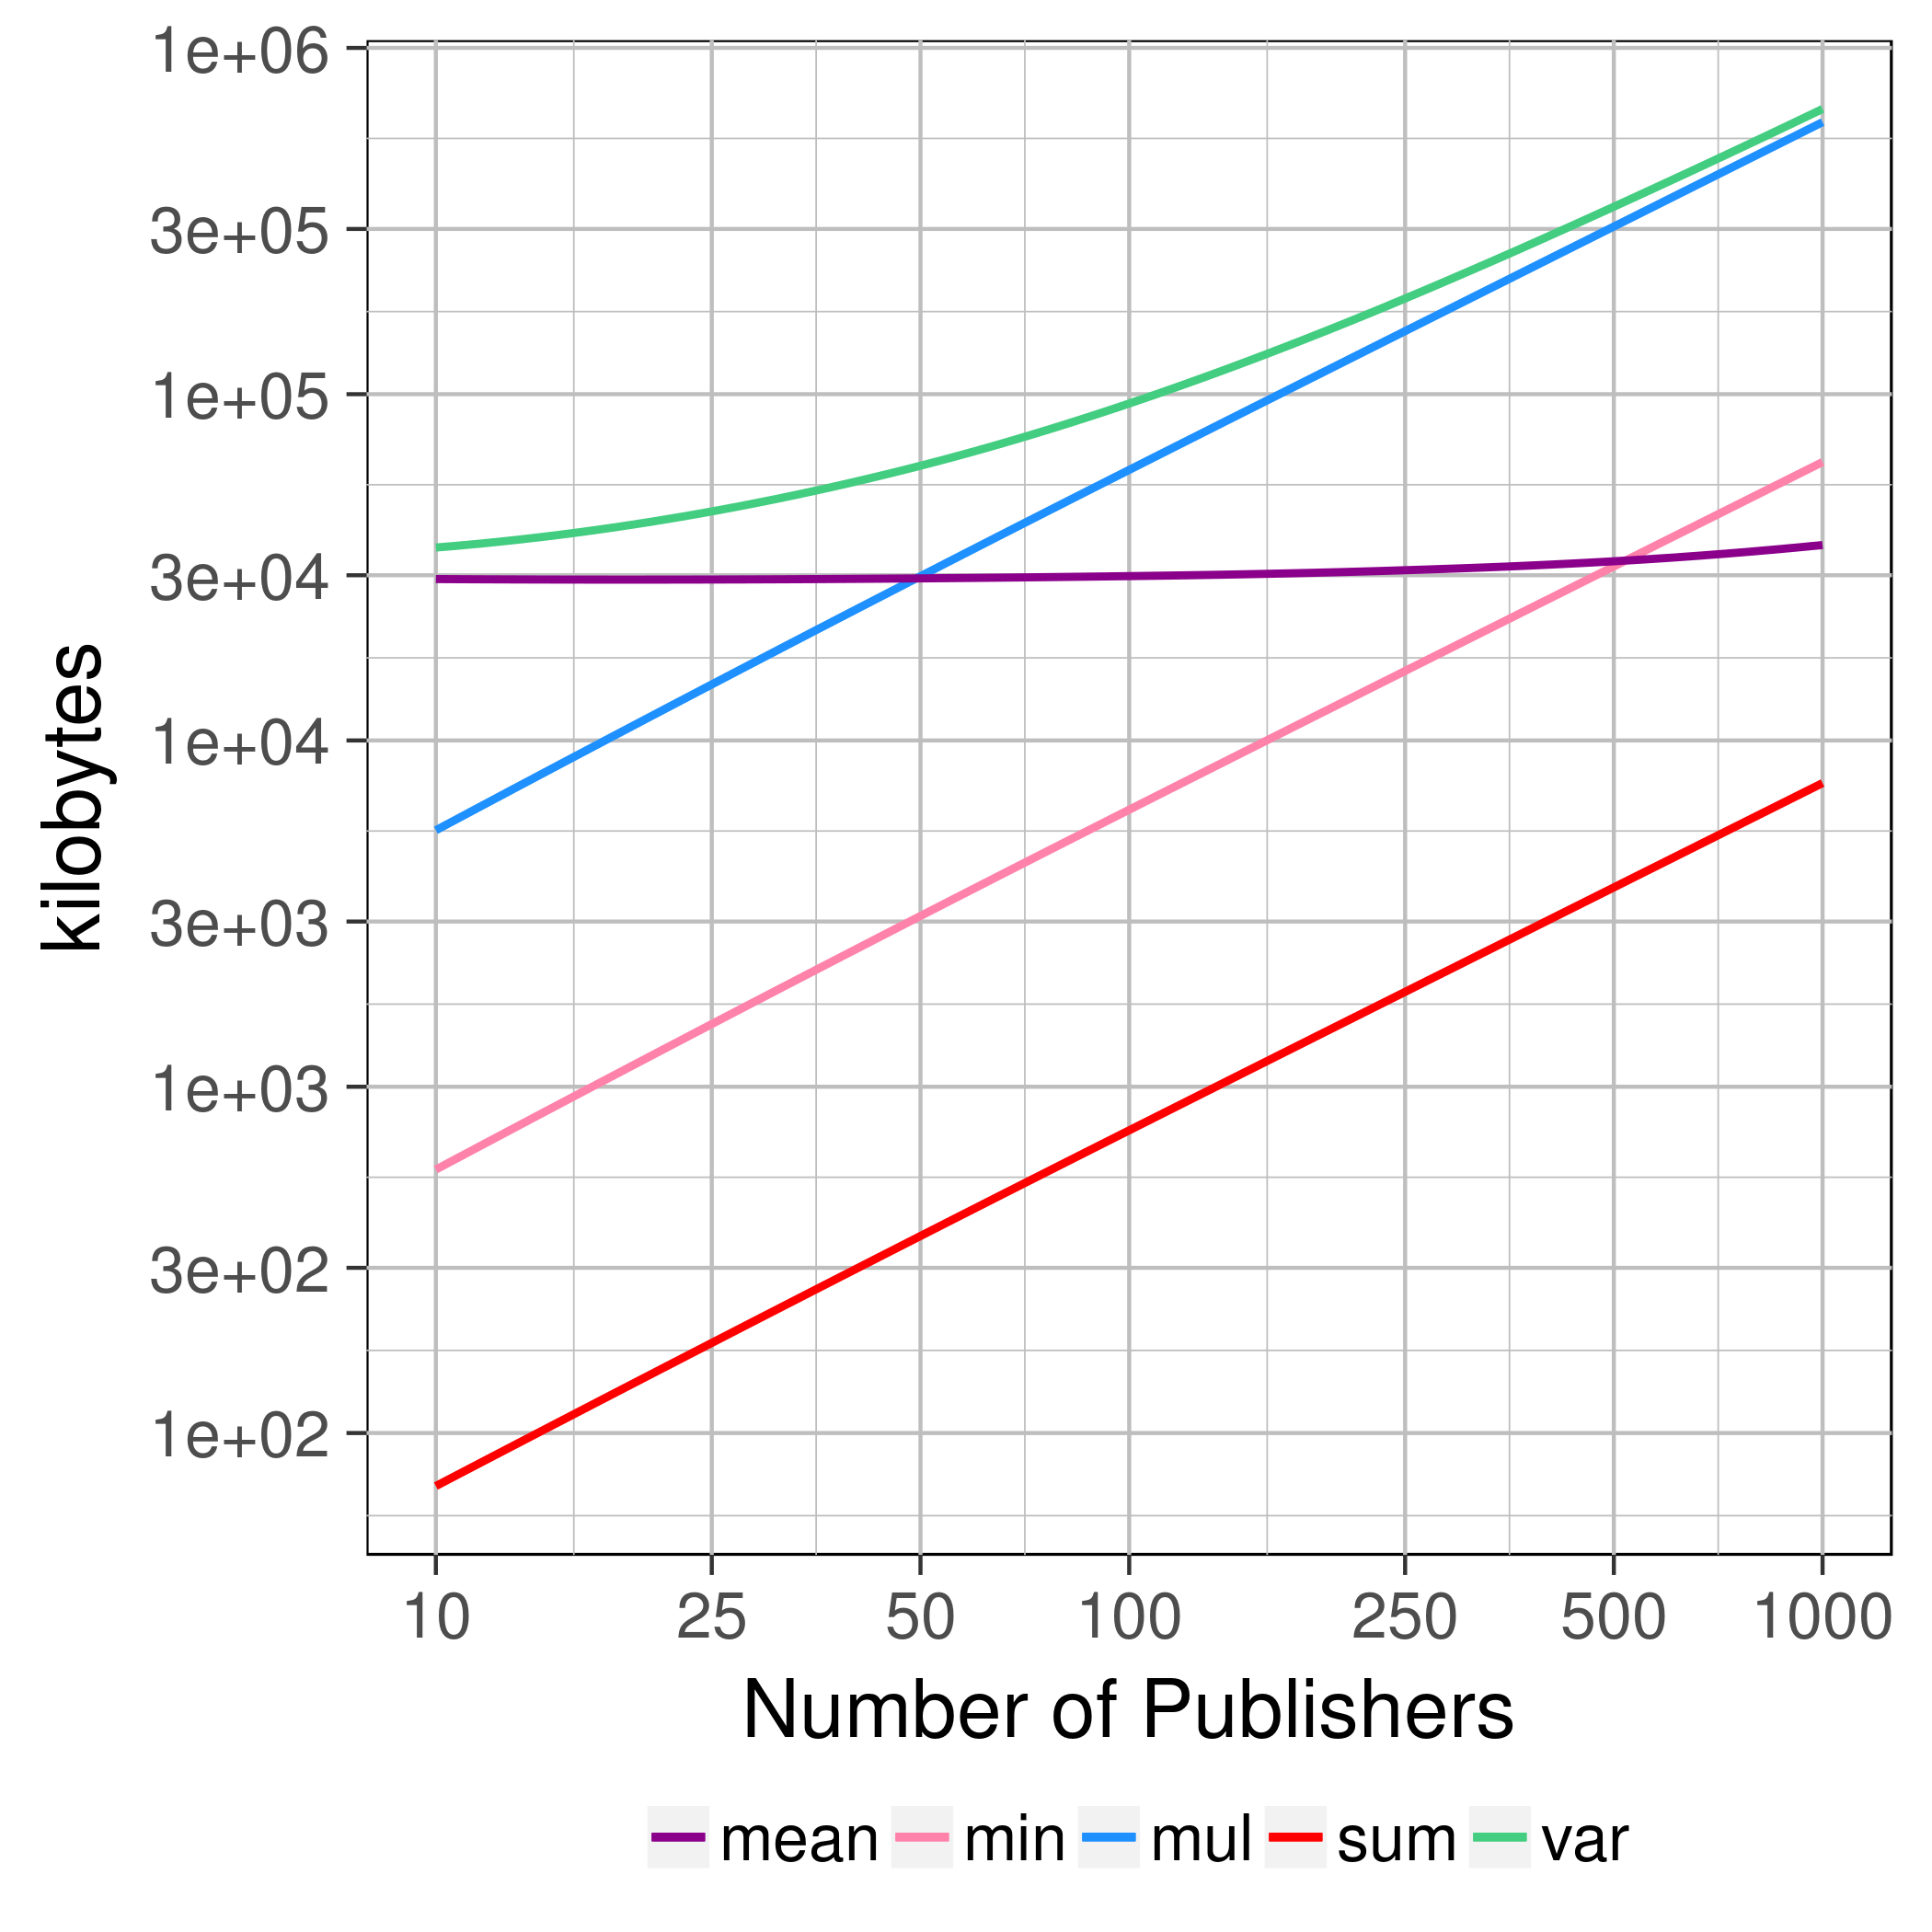
\includegraphics[width=0.5\textwidth]{plots/size_log.png}
  \caption{Size of the garbled circuit and the associated date required by the
  Broker to evaluate it.}
\end{figure}

\subsection{Applications}

% TODO: 1. Environmental Berkeley indor sensing data, correlation
\paragraph{Correlation of two data streams}

% TODO: 2. Road Volume sensor traffic, evaluation of the expected time to follow a path
\paragraph{Estimation of time required to follow a path with traffic}

% TODO: 3. LAX parking lot dataset, statistics
\paragraph{Continuous statistics of incoming data}

% TODO: 4. Turonet, wireless propagation constant, linear regression
\paragraph{One dimensional linear regression}

% TODO: 5. Smart bill, monthly electricity bill with different cost per hour of the day / threshold.

% Plots

% TODO: Discussion: bottlenecks.
% Sending the garbled circuit.
